% Chapter 4, Section 1: Overflow and Underflow

\section{Overflow and Underflow \difficultyInline{beginner}}
\label{sec:overflow-underflow}

Overflow and underflow are critical numerical issues that occur when computations produce values outside the representable range of floating-point arithmetic, causing catastrophic failures in deep learning algorithms that rely on precise numerical calculations.

\subsection{Intuition: The Problem with Finite Precision}

Imagine you're trying to measure the height of a building using a ruler that only has markings every meter. If the building is 10.7 meters tall, you might record it as 11 meters - you've lost some precision. Now imagine doing millions of calculations with this imprecise ruler, and you can see how small errors can compound into big problems. Computers face a similar challenge because they can only represent a finite number of digits, so they must round numbers, which is like having a ruler with limited markings where some information is always lost. In deep learning, this becomes critical because neural networks perform millions of calculations where small errors accumulate, exponential functions are common and can produce extremely large or small numbers, and gradients can become very small and might round to zero, breaking training. Computers represent real numbers with finite precision, typically using floating-point arithmetic, which leads to rounding errors that can accumulate and cause problems in deep learning algorithms.

\subsection{Floating-Point Representation}

The IEEE 754 standard defines floating-point numbers using a fixed number of bits to represent real numbers, with 32-bit floats having a smallest positive number of approximately $10^{-38}$, a largest number of approximately $10^{38}$, and a machine epsilon of approximately $10^{-7}$. This representation allows computers to handle a wide range of numbers but introduces limitations that can cause overflow when numbers exceed the maximum representable value and underflow when numbers become smaller than the minimum representable value.

\begin{figure}[h]
\centering
\begin{tikzpicture}
\begin{axis}[
    ylabel={Representable Numbers},
    xlabel={Value (log scale)},
    xmode=log,
    ymin=0,
    ymax=1,
    width=12cm,
    height=6cm,
    xtick={1e-40, 1e-30, 1e-20, 1e-10, 1, 1e10, 1e20, 1e30, 1e40},
    xticklabels={$10^{-40}$, $10^{-30}$, $10^{-20}$, $10^{-10}$, $1$, $10^{10}$, $10^{20}$, $10^{30}$, $10^{40}$},
    ytick=\empty
]
% Underflow region
\addplot[bookred, thick, domain=1e-50:1e-38] {0.2};
\node[bookred] at (axis cs: 1e-45, 0.3) {Underflow};

% Normal range
\addplot[bookpurple, thick, domain=1e-38:1e38] {0.5};
\node[bookpurple] at (axis cs: 1, 0.6) {Normal Range};

% Overflow region
\addplot[bookred, thick, domain=1e38:1e50] {0.8};
\node[bookred] at (axis cs: 1e45, 0.9) {Overflow};
\end{axis}
\end{tikzpicture}
\caption{Representable range for 32-bit floating-point numbers}
\label{fig:float-range}
\end{figure}

\subsection{Underflow}

\subsubsection{Intuition: When Numbers Become Too Small}

Think of underflow like trying to measure the width of a human hair with a ruler marked in meters. The hair is so thin that your ruler shows 0 meters - you've lost all information about the actual size.

In computers, \textbf{underflow} occurs when numbers become so small that they round to zero. This is like your ruler being too coarse to measure tiny objects.

\textbf{Underflow} occurs when numbers near zero are rounded to zero. This can be problematic when we need to compute ratios or logarithms. For example, the softmax function:

\begin{equation}
\text{softmax}(\vect{x})_i = \frac{\exp(x_i)}{\sum_j \exp(x_j)}
\end{equation}

can underflow if all $x_i$ are very negative.

\subsection{Overflow}

\subsubsection{Intuition: When Numbers Become Too Large}

Imagine trying to count the number of atoms in the universe using a calculator that can only display 8 digits. When you reach 99,999,999, the next number would be 100,000,000, but your calculator shows "Error" or resets to 0.

\textbf{Overflow} occurs when large numbers exceed representable values. In the softmax example, overflow can occur if some $x_i$ are very large.

\subsection{Numerical Stability}

To stabilize softmax, we use the identity:

\begin{equation}
\text{softmax}(\vect{x}) = \text{softmax}(\vect{x} - c)
\end{equation}

where $c = \max_i x_i$. This prevents both overflow and underflow.

Similarly, when computing $\log(\sum_i \exp(x_i))$, we use the \textbf{log-sum-exp} trick:

\begin{equation}
\log\left(\sum_i \exp(x_i)\right) = c + \log\left(\sum_i \exp(x_i - c)\right)
\end{equation}

\subsubsection{Example: Softmax Numerical Issues}

Consider computing softmax for $\vect{x} = [1000, 1001, 1002]$:

\textbf{Naive approach:}
\begin{align}
\exp(1000) &\approx \infty \quad \text{(overflow!)} \\
\exp(1001) &\approx \infty \quad \text{(overflow!)} \\
\exp(1002) &\approx \infty \quad \text{(overflow!)} \\
\text{softmax}(\vect{x}) &= [\text{NaN}, \text{NaN}, \text{NaN}]
\end{align}

\textbf{Stable approach:}
\begin{align}
c &= \max(1000, 1001, 1002) = 1002 \\
\exp(1000-1002) &= \exp(-2) \approx 0.135 \\
\exp(1001-1002) &= \exp(-1) \approx 0.368 \\
\exp(1002-1002) &= \exp(0) = 1.000 \\
\text{softmax}(\vect{x}) &= [0.090, 0.245, 0.665]
\end{align}

\begin{figure}[h]
\centering
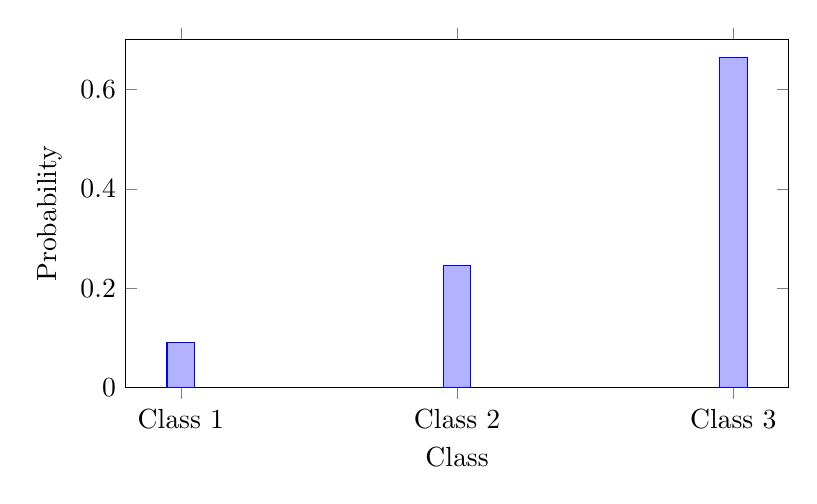
\begin{tikzpicture}
\begin{axis}[
    ylabel={Probability},
    xlabel={Class},
    ybar,
    ymin=0,
    ymax=0.7,
    width=10cm,
    height=6cm,
    xtick={1,2,3},
    xticklabels={Class 1, Class 2, Class 3}
]
\addplot coordinates {(1,0.090) (2,0.245) (3,0.665)};
\end{axis}
\end{tikzpicture}
\caption{Stable softmax computation for large inputs}
\label{fig:stable-softmax}
\end{figure}

\subsection{Other Numerical Issues}

Beyond overflow and underflow, several other numerical issues can affect deep learning computations. Catastrophic cancellation occurs when subtracting nearly equal numbers, leading to loss of precision that can significantly impact gradient calculations and model training. Accumulated rounding errors represent another critical concern where small errors compound through many operations, potentially causing the model to converge to suboptimal solutions or fail to train entirely. To address these issues, several solutions can be employed including using higher precision arithmetic with 64-bit floats to reduce rounding errors, implementing algorithmic modifications like the log-sum-exp trick to maintain numerical stability, applying batch normalization to stabilize activations and gradients, and using gradient clipping to prevent exploding gradients that can cause numerical instability during training.
